\chapter{Lektion 5}

\section{Kapitel 9}
Udbetalling afhænger af mange ting, handling, tid mm. Her vil der ses på hvordan få principper i spilteori kan hjælpe os med at forstå handlingen fra oligopolister og monopolistisk konkurrenter. 

\subsection{Using game theory to analyse strategic decisions}
I ethvert spil afhænger dit træk af hvordan din modstander reagere på det, og derfor går det ud på at kende din modstanders næste træk. 

\subsubsection{The three elements of a game}
Det er tre \textbf{basis elementer} i et spil: spillerne, mulige "træk og strategier" og de udbetallinger spillerne kan få ved et træk. 

\begin{eks} \textbf{} %Nyt eksempel
\newline
Antag at United Airline og American Airlines var de eneste på Chicago-St Louis ruten. Hver har en økonomisk profit på 6.000kr per flyafgang. Hvis en af dem hæver reklame omkostningerne med 1000kr, vil deres profit stige til 8.000kr mens modstanderens profit vil falde til 2.000 kr. Hvis begge hæver reklameomkostningerne med 1.000kr vil begges profit falde til 5.500kr. 

\textbf{Basiselementerne:} De to flyselskaber, strategierne er at bruge mere eller ikke bruge mere på reklameomkostningerne, udbetalingerne er de fire forskellige mulige udfald ud fra valget om reklameomkostningerne. Disse kan ses på \textbf{udbetalings matricen} nedenfor.

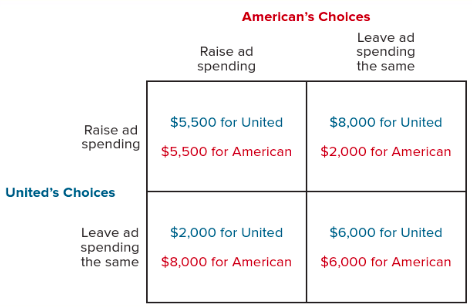
\includegraphics[scale=0.4]{Afsnit/Lektion5/udbetalingsmatrice.png}

\textbf{Dominant strategi} er en strategi der giver en højere udbetaling lige meget hvad andre spillere vælger. Alle andre strategier end denne er de \textbf{dominerede strategier}. I dette tilfælde vil man formentlig vælge ikke at bruge mere, da man vil forvente at hvis en hæver reklameomkostningerne vil den anden også hæve reklameomkostningerne da de ikke er interesseret i en mindre profit. Her vil begge parter tjene mindre end hvis de bare lader reklameomkostningerne forblive på det samme niveau. \end{eks}

\subsubsection{Nash Equilibrium}
Et spil siges at være i ligevægt hvis alle spilleres strategier er det bedste de kan vælge givet andre spilleres valg. Dette kaldes \textbf{Nash ligevægt}. Når dette er opnået er der ingen af spillerne der ville få noget ud af at ændre strategi. Hvis der er en dominant strategi, vil ligevægten være der hvis begge parter følger denne. Man kan stadig nå ligevægt selvom der ikke findes en dominant strategi, det vigtige er bare at hvis man er i ligevægt, vil man tabe noget nogen anden vælger en anden strategi. 

\subsection{The prisoner's dilemma}
\textbf{Fangens dilemma} er når alle spillere vælger den dominante strategi og dette resulterer i en lavere udbetaling end hvis man valgte en domineret strategi. 

\subsubsection{The original prisoner's dilemma}
Se side 242-243, det giver mening. De snakker bare om to fanger der har samme problem som de to flyselskaber. 

\subsubsection{The economics of cartels}
\textbf{Et kartel} er ethvert koalition/forening af firmaer der begrænser produktionen for at få højere økonomisk profit. Kartel dannelse er et klassisk eksempel på hvordan fangernes dilemma kan opstå.

\begin{eks} \textbf{} %Nyt eksempel
\newline
To firmaer sælger vand og vælger at forme et kartel så de kun producere halvdelen af deres normale produktion og sælger til monopolpriser. Da aftalen ikke er lovligt lavet er der ikke noget der stopper den ene producent fra at sælge til en lavere pris, og dermed få hele markedet. Producenternes udbetalings matrice ses nedenunder.

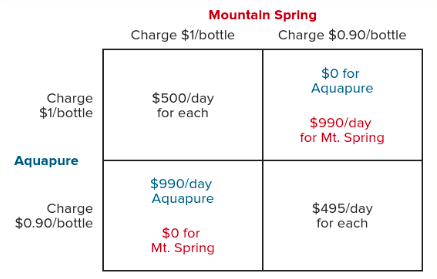
\includegraphics[scale=0.7]{Afsnit/Lektion5/udbetalingsmatriceforvand.png}

Hvert firma ved at ved at sætte prisen en smule ned kan de vinde hele markedet tilbage og få en temmelig højere økonomisk profit. Her vil det andet firma svarer igen og den samlede profit for dem begge vil falde. Dette kan forsætte til de når marginalomkostningerne. Derfor er karteldannelse historisk kendt for at være ustabile. 
\end{eks}

\subsubsection{Tit-for-tat and the repeated prisoner's dilemma}
Når der er nogen firmaer der er i fangernes dilemma flere gange med hinanden kan man lede efter måde at "straffe" et firma hvis de afviger. Når firmaer er i fangernes dilemma med hinanden flere gange, kaldes det for \textbf{gentagne fangernes dilemma.} Der er en strategi der har bevist sig meget nyttig i disse situationer, det kaldes for \textbf{tit-for-tat}. Det går ud på at man gør det "modstanderen" gjorde sidste gang. Dette gør at firmaer ikke afviger da dette vil blive straffet med "hævn" næste gang. Dette virker dog kun når der er to firmaer. 

Nogle gange kommer profitten også an på tidspunktet man udvikler eller laver sit træk. Dette kan beskrives ved et \textbf{beslutnings træ} eller \textbf{spil træ}. Dette ses nedenunder, hvor det er to bilforhandlere der skal beslutte om de skal udvikle en hybrid model. 

\includegraphics[scale=0.5]{Afsnit/Lektion5/spiltræ.png}

Her har Dodge førstevalg, og skal self vælge at lave en hybrid da Chevrolet så vælger ikke at lave en fordi det vil give størst mulig profit. 

\subsubsection{Credible threats and promises}
En \textbf{troværdig trussel} er en hvor den der truer's interesse er at føre truslen ud i livet når tiden kommer. På samme måde er der også \textbf{troværdige løfter}.

\subsubsection{Monopolistic competition when location matters}
Selvom det tit er tilfældet at den der har det første træk har en fordel, gælder dette ikke altid. 

\begin{eks} %Nyt eksempel
\newline
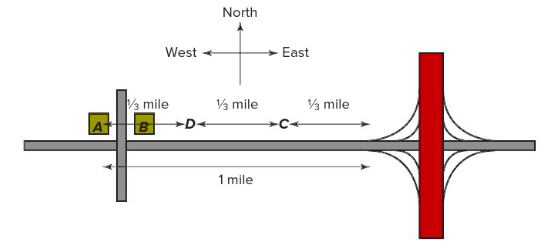
\includegraphics[scale=0.6]{Afsnit/Lektion5/motorvej.png}

Her ses det at A først vælger at have en butik og derefter er der en ny der åbner en butik B. Kunderne tager den butik der er tættest på dem og derfor vil B nu få alle kunderne hen til motorvejen(rød) istedet for A. Derudover vil B aldrig ligge sig ved punktet C da mellem C og A ville kun den halvdel af kunder der lå tættest på C handle der, resten ville gå i A. Det er også derfor at butikker tit er i grupper. 
\end{eks}

For mange firmaer er det ikke bare forskellen på lokation der spiller en rolle, men forskellen på timing, fx programmer skal sendes kl 20, da der er der flest ser dem. 

\subsection{Commitment problems}
Når firmaer (som i fangernes dilemma) er i en situation hvor de har problemer med at opnå det ønskede resultat fordi de hverken kan lave troværdige løfter eller trusler står de i et \textbf{forpligtelses problem}. Dette kan løses ved at man finder et \textbf{forpligtelses apperat} - noget der gør at de har "opmuntring" til at holde deres løfter. 

\begin{eks} \textbf{} %Nyt eksempel
\newline
Der er en ejer af en resturant. Hun vil have tjenerne til at yde god service for kunderne så de kommer igen. Fordi det er vigtigt for hende vil hun gerne give lidt mere i løn for at sikre det. Tjenerne vil yde god service hvis de får mere. Problemet er at ejeren ikke kan overvåge personalet og derfor ikke kan sikre at de holder løftet. Hvis hun ikke finder en måde at sikre sig at tjenerne yder god service vil hun ikke betale dem ekstra. Ved at kunderne skal betale drikkepenge til tjenerne hvis de har ydet god service, på denne måde ved ejeren hvem der er gode og tjenerne har en grund til at yde god service.  
\end{eks}

\subsubsection{Solving commitment problems with psychological incentives}








